% MigrationBench figure: preserve the supplied Coordinates -> Descriptors ->
% atomic-species neural networks -> Total Energy visual pipeline, while adding
% two coordinate distributions and three explicit training/model routes.

\documentclass[tikz,border=0pt]{standalone}
\usepackage{tikz}
\usetikzlibrary{arrows.meta}
\usepackage{amsmath,amssymb}
\usepackage{helvet}
\renewcommand{\familydefault}{\sfdefault}

\definecolor{ink}{HTML}{072B45}
\definecolor{arrowblue}{HTML}{156982}
\definecolor{atomorange}{HTML}{E9782E}
\definecolor{atomviolet}{HTML}{A12B91}
\definecolor{inputblue}{HTML}{0A7FC2}
\definecolor{coordblue}{HTML}{0F6F8F}
\definecolor{hiddenorange}{HTML}{F1A247}
\definecolor{outputviolet}{HTML}{7030A0}
\definecolor{rulegray}{HTML}{D6E0E5}
\definecolor{muted}{HTML}{667985}
\definecolor{softblue}{HTML}{EFF7FB}
\definecolor{softorange}{HTML}{FFF6E8}
\definecolor{softpurple}{HTML}{F6F0FA}

\tikzset{
  title/.style={font=\sffamily\fontsize{9.0}{10.5}\selectfont,align=center,inner sep=0pt},
  stage/.style={font=\sffamily\fontsize{8.0}{9.3}\selectfont,align=center,inner sep=0pt},
  label/.style={font=\sffamily\fontsize{6.5}{7.6}\selectfont,align=center,inner sep=0pt},
  tiny/.style={font=\sffamily\fontsize{5.6}{6.6}\selectfont,align=center,inner sep=0pt},
  mathlabel/.style={font=\rmfamily\fontsize{7.0}{8.0}\selectfont,inner sep=0pt},
  atom/.style={circle,draw=ink,line width=0.7pt,minimum size=5.2pt,inner sep=0pt},
  neuron/.style={circle,draw=ink,line width=0.75pt,minimum size=9.0pt,inner sep=0pt},
  mini/.style={circle,draw=ink,line width=0.6pt,minimum size=5.7pt,inner sep=0pt},
  routepill/.style={rounded corners=3pt,draw=ink,line width=0.75pt,fill=softorange,
    minimum width=23mm,minimum height=9mm,inner sep=1.5pt,align=center,
    font=\sffamily\fontsize{5.8}{6.8}\selectfont},
  checkpoint/.style={circle,draw=ink,line width=0.7pt,fill=outputviolet,
    minimum size=8.0pt,inner sep=0pt},
}

\newcommand{\flow}[2]{%
  \draw[arrowblue,line width=1.2pt,-{Latex[length=4.1pt,width=3.0pt]}] (#1) -- (#2);%
}
\newcommand{\thinflow}[2]{%
  \draw[arrowblue,line width=0.82pt,-{Latex[length=3.2pt,width=2.4pt]}] (#1) -- (#2);%
}
\newcommand{\dashflow}[2]{%
  \draw[ink!75,line width=0.62pt,dashed,-{Latex[length=3.0pt,width=2.2pt]}] (#1) -- (#2);%
}

% A compact, real node-and-connection network glyph for each route.
\newcommand{\miniNN}[2]{%
  \begin{scope}[shift={(#1,#2)}]
    \foreach \y in {22,0,-22} {\foreach \z in {18,0,-18}{\draw[ink,line width=0.45pt] (0,\y) -- (28,\z);}}
    \foreach \y in {18,0,-18} {\draw[ink,line width=0.45pt] (28,\y) -- (54,0);}
    \foreach \y in {22,0,-22} {\node[mini,fill=inputblue] at (0,\y) {};}
    \foreach \y in {18,0,-18} {\node[mini,fill=hiddenorange] at (28,\y) {};}
    \node[mini,fill=outputviolet] at (54,0) {};
  \end{scope}%
}

\begin{document}
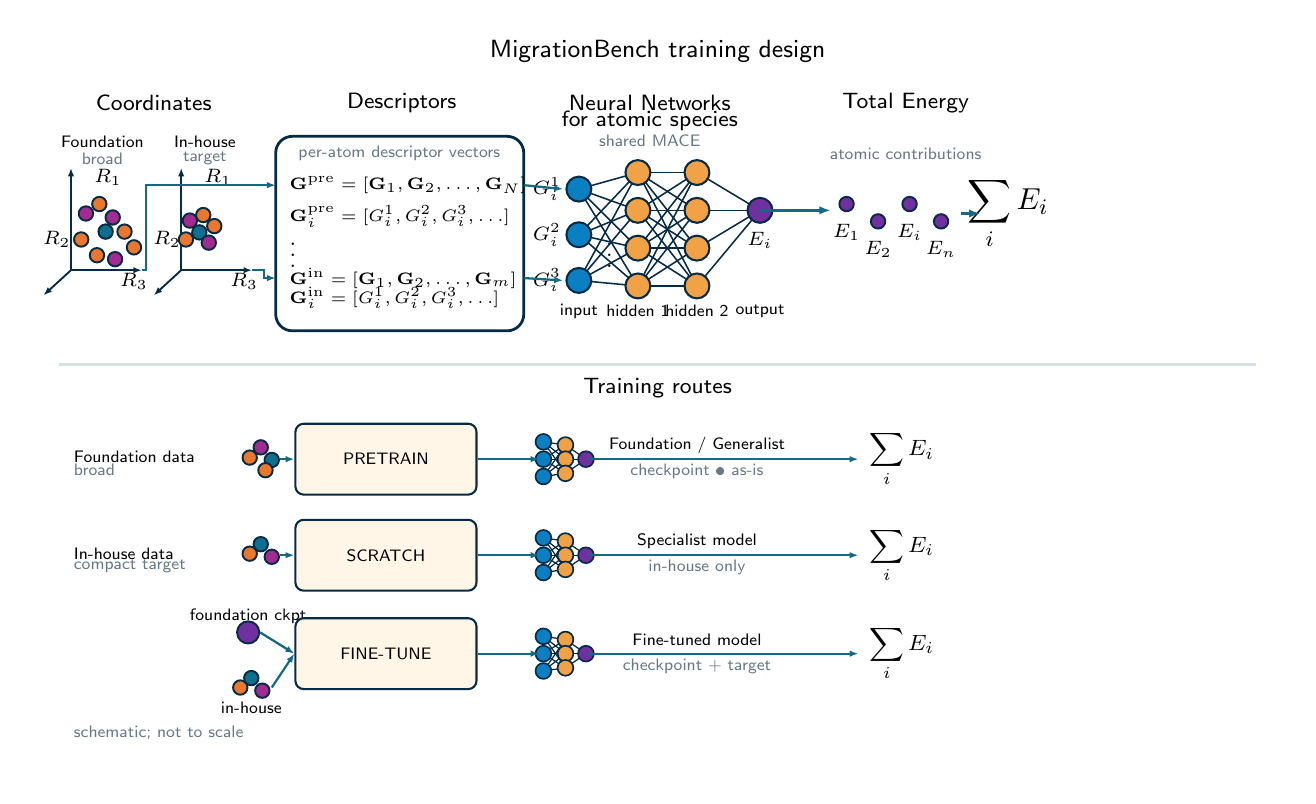
\begin{tikzpicture}[x=0.1mm,y=0.1mm]
  \path[use as bounding box] (0,0) rectangle (1600,950);

  % Title and the four original scientific stages.
  \node[title] at (800,920) {MigrationBench training design};
  \node[stage] at (160,855) {Coordinates};
  \node[stage] at (475,855) {Descriptors};
  \node[stage] at (790,855) {Neural Networks};
  \node[stage] at (790,831) {for atomic species};
  \node[tiny,text=muted] at (790,807) {shared MACE};
  \node[stage] at (1115,855) {Total Energy};

  % --------------------------------------------------------------------------
  % UPPER BAND: the original four visual modules, with two coordinate inputs.
  % --------------------------------------------------------------------------
  % Two coordinate tripods, side-by-side, to keep the comparison immediate.
  \node[label] at (95,805) {Foundation};
  \node[tiny,text=muted] at (95,784) {broad};
  \draw[ink,line width=0.68pt,-{Latex[length=3.1pt,width=2.3pt]}] (55,642) -- (55,772);
  \draw[ink,line width=0.68pt,-{Latex[length=3.1pt,width=2.3pt]}] (55,642) -- (145,642);
  \draw[ink,line width=0.68pt,-{Latex[length=3.1pt,width=2.3pt]}] (55,642) -- (20,610);
  \node[mathlabel] at (37,681) {$R_2$};
  \node[mathlabel] at (102,760) {$R_1$};
  \node[mathlabel] at (135,628) {$R_3$};
  \node[atom,fill=atomviolet] at (74,714) {};
  \node[atom,fill=atomorange] at (91,726) {};
  \node[atom,fill=atomviolet] at (108,709) {};
  \node[atom,fill=atomorange] at (123,691) {};
  \node[atom,fill=atomorange] at (68,681) {};
  \node[atom,fill=atomorange] at (88,661) {};
  \node[atom,fill=atomviolet] at (111,656) {};
  \node[atom,fill=coordblue] at (99,691) {};
  \node[atom,fill=atomorange] at (135,671) {};

  \node[label] at (225,805) {In-house};
  \node[tiny,text=muted] at (225,784) {target};
  \draw[ink,line width=0.68pt,-{Latex[length=3.1pt,width=2.3pt]}] (195,642) -- (195,772);
  \draw[ink,line width=0.68pt,-{Latex[length=3.1pt,width=2.3pt]}] (195,642) -- (285,642);
  \draw[ink,line width=0.68pt,-{Latex[length=3.1pt,width=2.3pt]}] (195,642) -- (160,610);
  \node[mathlabel] at (177,681) {$R_2$};
  \node[mathlabel] at (242,760) {$R_1$};
  \node[mathlabel] at (275,628) {$R_3$};
  \node[atom,fill=atomviolet] at (206,705) {};
  \node[atom,fill=atomorange] at (223,712) {};
  \node[atom,fill=atomorange] at (237,698) {};
  \node[atom,fill=coordblue] at (218,690) {};
  \node[atom,fill=atomviolet] at (230,677) {};
  \node[atom,fill=atomorange] at (201,681) {};

  % Descriptor matrix/vector representation.
  \draw[ink,line width=1.0pt,rounded corners=6pt] (315,565) rectangle (630,812);
  \node[tiny,text=muted] at (472,790) {per-atom descriptor vectors};
  \node[mathlabel,anchor=west,font=\rmfamily\fontsize{6.0}{7.0}\selectfont]
    at (332,750) {$\mathbf{G}^{\rm pre}=[\mathbf{G}_1,\mathbf{G}_2,\ldots,\mathbf{G}_N]$};
  \node[mathlabel,anchor=west,font=\rmfamily\fontsize{6.0}{7.0}\selectfont]
    at (332,710) {$\mathbf{G}^{\rm pre}_i=[G_i^1,G_i^2,G_i^3,\ldots]$};
  \node[mathlabel,anchor=west,font=\rmfamily\fontsize{8.5}{9}\selectfont]
    at (332,672) {$\vdots\hspace{112pt}\vdots$};
  \node[mathlabel,anchor=west,font=\rmfamily\fontsize{6.0}{7.0}\selectfont]
    at (332,632) {$\mathbf{G}^{\rm in}=[\mathbf{G}_1,\mathbf{G}_2,\ldots,\mathbf{G}_m]$};
  \node[mathlabel,anchor=west,font=\rmfamily\fontsize{6.0}{7.0}\selectfont]
    at (332,607) {$\mathbf{G}^{\rm in}_i=[G_i^1,G_i^2,G_i^3,\ldots]$};
  % Independent provenance arrows: each coordinate panel feeds its own
  % descriptor row rather than appearing to originate from a shared placeholder.
  \draw[arrowblue,line width=0.82pt,-{Latex[length=3.2pt,width=2.4pt]}]
    (145,642) -- (150,642) -- (150,750) -- (315,750);
  \draw[arrowblue,line width=0.82pt,-{Latex[length=3.2pt,width=2.4pt]}]
    (285,642) -- (300,642) -- (300,632) -- (315,632);

  % Full atomic-species neural network, retaining the original element.
  \foreach \i in {1,2,3} {
    \foreach \j in {1,2,3,4} {
      \draw[ink,line width=0.56pt] (700,{745-(\i-1)*58}) -- (775,{766-(\j-1)*48});
    }
  }
  \foreach \i in {1,2,3,4} {
    \foreach \j in {1,2,3,4} {
      \draw[ink,line width=0.56pt] (775,{766-(\i-1)*48}) -- (850,{766-(\j-1)*48});
    }
  }
  \foreach \i in {1,2,3,4} {\draw[ink,line width=0.56pt] (850,{766-(\i-1)*48}) -- (930,718);}
  \foreach \y in {745,687,629} {\node[neuron,fill=inputblue] at (700,\y) {};}
  \foreach \y in {766,718,670,622} {
    \node[neuron,fill=hiddenorange] at (775,\y) {};
    \node[neuron,fill=hiddenorange] at (850,\y) {};
  }
  \node[neuron,fill=outputviolet] at (930,718) {};
  \node[mathlabel,anchor=east] at (678,745) {$G_i^1$};
  \node[mathlabel,anchor=east] at (678,687) {$G_i^2$};
  \node[mathlabel,anchor=east] at (678,629) {$G_i^3$};
  \node[mathlabel] at (930,680) {$E_i$};
  \node[tiny] at (700,590) {input};
  \node[tiny] at (775,590) {hidden 1};
  \node[tiny] at (850,590) {hidden 2};
  \node[tiny] at (930,590) {output};
  \thinflow{630,750}{680,745}
  \thinflow{630,632}{680,629}

  % Explicit atomic-energy contributions and total-energy aggregation.
  \node[tiny,text=muted] at (1115,790) {atomic contributions};
  \node[atom,fill=outputviolet] at (1040,726) {};
  \node[atom,fill=outputviolet] at (1080,704) {};
  \node[atom,fill=outputviolet] at (1120,726) {};
  \node[atom,fill=outputviolet] at (1160,704) {};
  \node[mathlabel] at (1040,690) {$E_1$};
  \node[mathlabel] at (1080,668) {$E_2$};
  \node[mathlabel] at (1120,690) {$E_i$};
  \node[mathlabel] at (1160,668) {$E_n$};
  \node[font=\rmfamily\fontsize{11}{13}\selectfont,inner sep=0pt] (etotal) at (1245,714) {$\displaystyle\sum_i E_i$};
  \flow{930,718}{1020,718}
  \flow{1185,714}{1210,714}

  % Divider between preserved scientific pipeline and training design.
  \draw[rulegray,line width=0.9pt] (40,522) -- (1560,522);
  \node[stage] at (800,492) {Training routes};

  % --------------------------------------------------------------------------
  % LOWER BAND: actual route sources, operations, mini network glyphs, and
  % energy outputs.  These replace placeholder MACE/model cards.
  % --------------------------------------------------------------------------
  % Route 1: Generalist / foundation.
  \node[label,anchor=west] at (58,405) {Foundation data};
  \node[tiny,text=muted,anchor=west] at (58,389) {broad};
  \node[atom,fill=atomorange] at (282,404) {};
  \node[atom,fill=atomviolet] at (296,417) {};
  \node[atom,fill=coordblue] at (310,401) {};
  \node[atom,fill=atomorange] at (302,388) {};
  \node[routepill] (pre) at (455,402) {PRETRAIN};
  \thinflow{320,402}{pre.west}
  \miniNN{655}{402}
  \thinflow{pre.east}{650,402}
  \node[label] at (850,420) {Foundation / Generalist};
  \node[tiny,text=muted] at (850,386) {checkpoint \textbullet{} as-is};
  \node[font=\rmfamily\fontsize{8.5}{10}\selectfont,inner sep=0pt] at (1110,402) {$\displaystyle\sum_i E_i$};
  \thinflow{710,402}{1055,402}

  % Route 2: Specialist / scratch.
  \node[label,anchor=west] at (58,282) {In-house data};
  \node[tiny,text=muted,anchor=west] at (58,266) {compact target};
  \node[atom,fill=atomorange] at (282,282) {};
  \node[atom,fill=coordblue] at (296,294) {};
  \node[atom,fill=atomviolet] at (310,278) {};
  \node[routepill] (scratch) at (455,280) {SCRATCH};
  \thinflow{320,280}{scratch.west}
  \miniNN{655}{280}
  \thinflow{scratch.east}{650,280}
  \node[label] at (850,298) {Specialist model};
  \node[tiny,text=muted] at (850,264) {in-house only};
  \node[font=\rmfamily\fontsize{8.5}{10}\selectfont,inner sep=0pt] at (1110,280) {$\displaystyle\sum_i E_i$};
  \thinflow{710,280}{1055,280}

  % Route 3: Fine-tuning / two inputs.
  \node[checkpoint] (routeckpt) at (280,182) {};
  \node[tiny] at (280,202) {foundation ckpt};
  \node[atom,fill=atomorange] at (270,112) {};
  \node[atom,fill=coordblue] at (284,124) {};
  \node[atom,fill=atomviolet] at (298,108) {};
  \node[tiny] at (284,86) {in-house};
  \node[routepill] (fine) at (455,155) {FINE-TUNE};
  \thinflow{routeckpt.east}{fine.west}
  \thinflow{310,112}{fine.west}
  \miniNN{655}{155}
  \thinflow{fine.east}{650,155}
  \node[label] at (850,173) {Fine-tuned model};
  \node[tiny,text=muted] at (850,139) {checkpoint + target};
  \node[font=\rmfamily\fontsize{8.5}{10}\selectfont,inner sep=0pt] at (1110,155) {$\displaystyle\sum_i E_i$};
  \thinflow{710,155}{1055,155}

  \node[tiny,text=muted,anchor=west] at (58,55) {schematic; not to scale};
\end{tikzpicture}
\end{document}
